% ===========================================================================
% Figura 1.2: Fuentes de error de sincronización
% Basada en la Figura 1.2 del documento base
% ===========================================================================
\documentclass[tikz,border=10pt]{standalone}
\usepackage[utf8]{inputenc}
\usepackage[T1]{fontenc}
\usepackage{lmodern}
\usepackage{amsmath}
\usetikzlibrary{shapes.geometric, arrows.meta, positioning, fit}

\begin{document}
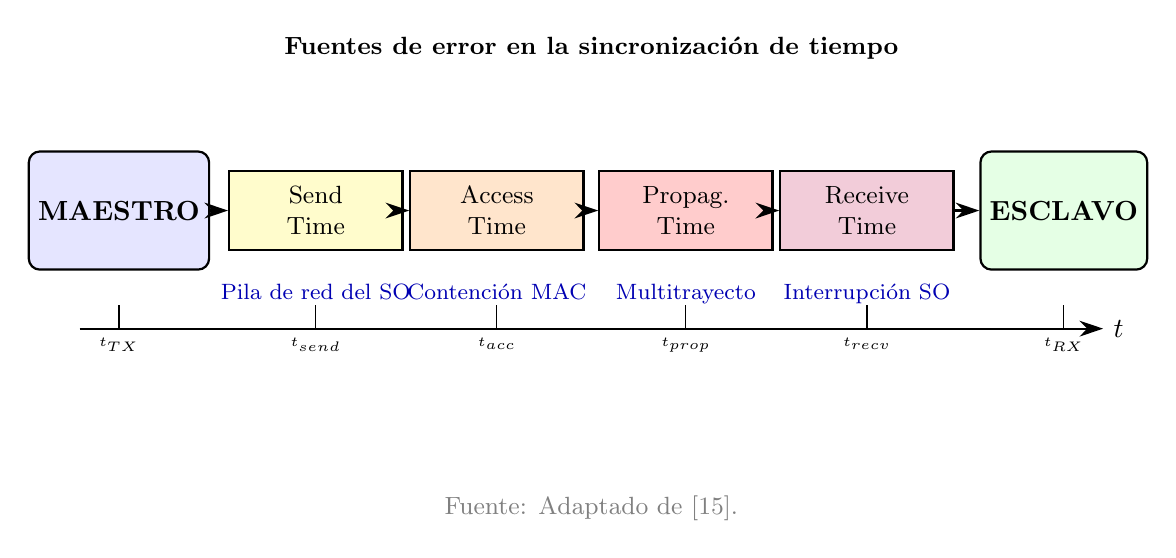
\begin{tikzpicture}[
    block/.style={rectangle, draw, thick, minimum width=2.2cm, minimum height=1cm, align=center, font=\small},
    arrow/.style={-{Stealth[length=3mm,width=2mm]}, thick},
    label/.style={font=\footnotesize, align=center}
  ]

  % Nodos maestro y esclavo
  \node[draw, thick, rounded corners, fill=blue!10, minimum width=2cm, minimum height=1.5cm] (master) at (0,0) {\textbf{MAESTRO}};
  \node[draw, thick, rounded corners, fill=green!10, minimum width=2cm, minimum height=1.5cm] (slave) at (12,0) {\textbf{ESCLAVO}};

  % Bloques de retardo intermedios
  \node[block, fill=yellow!20] (send) at (2.5,0) {Send\\Time};
  \node[block, fill=orange!20] (access) at (4.8,0) {Access\\Time};
  \node[block, fill=red!20] (prop) at (7.2,0) {Propag.\\Time};
  \node[block, fill=purple!20] (recv) at (9.5,0) {Receive\\Time};

  % Flechas entre bloques
  \draw[arrow] (master.east) -> (send.west);
  \draw[arrow] (send.east) -> (access.west);
  \draw[arrow] (access.east) -> (prop.west);
  \draw[arrow] (prop.east) -> (recv.west);
  \draw[arrow] (recv.east) -> (slave.west);

  % Línea de tiempo
  \draw[thick, -{Stealth[length=3mm,width=2mm]}] (-0.5,-1.5) -- (12.5,-1.5) node[right] {$t$};

  % Etiquetas de timeline
  \foreach \x/\txt in {0/{$t_{TX}$},2.5/{$t_{send}$},4.8/{$t_{acc}$},7.2/{$t_{prop}$},9.5/{$t_{recv}$},12/{$t_{RX}$}} {
    \draw (\x,-1.5) -- (\x,-1.2);
    \node[below, font=\tiny] at (\x,-1.5) {\txt};
  }

  % Descripciones debajo
  \node[below=0.3cm, label, text=blue!70!black] at (send.south) {Pila de red del SO};
  \node[below=0.3cm, label, text=blue!70!black] at (access.south) {Contención MAC};
  \node[below=0.3cm, label, text=blue!70!black] at (prop.south) {Multitrayecto};
  \node[below=0.3cm, label, text=blue!70!black] at (recv.south) {Interrupci\'on SO};

  % Título
  \node[above=0.3cm, font=\small\bfseries] at (6,1.5) {Fuentes de error en la sincronización de tiempo};

  \node[font=\small, text=gray, below] at (6,-3.5) {Fuente: Adaptado de [15].};
\end{tikzpicture}
\end{document}
